%\documentclass{book}
%\usepackage[subpreambles=false]{standalone}

%%%%%%%%%%%%%%%%%%%%%%%%%%%
% Silence warning messages
\usepackage{silence}
\WarningsOff[scrlayer-notecolumn]
\WarningsOff[biblatex]

%%%%%%%%%%%%%%%%%%%%
% Commenting

%\usepackage[author=Lyndon]{pdfcomment}
%\newcommand{\pdfcomment}[1]{} %ignore all comments

%\usepackage{todonotes}
%\newcommand{\pdfcomment}{\todo}


%%%%%%%%%%%%%%%%%%%%
% Tables
\usepackage{booktabs}

%%%%%%%%%%%%%%%%%%%
% Fonts
\usepackage{tgadventor} %sans
\usepackage{tgpagella}  %serif
\usepackage{inconsolata} %mono
\usepackage[T1]{fontenc}

\usepackage{microtype}
\usepackage[all]{nowidow}
%%%%%%%%%%%%%%%%%%%%%%%
% Styling
\setcounter{secnumdepth}{4}
\setcounter{tocdepth}{2}

\usepackage{placeins}



%%%%%%%%%%%%%%%%%%%
% Math
\usepackage{amsmath, amssymb, stmaryrd, mathtools}
\DeclareMathOperator*{\argmin}{argmin}
\DeclareMathOperator*{\argmax}{argmax}

\usepackage{xparse,xstring,etoolbox}
% crossref this against notation section
\newcommand{\vv}[1]{\tilde{#1}} % vector
\newcommand{\seq}[1]{\mathcal{#1}} % sequence
\newcommand{\set}[1]{\mathbb{#1}} % set

%%%%%%%%%
% Indexing/sequence indexing
\newcommand{\seqind}[2]{#1^{#2}} % seqence index
\newcommand{\ind}[2]{#1_{#2}} % indexed
\newcommand{\disamb}[2]{#1^{\mathrm{#2}}} %disambiguated

%% Smart indexing and naming
\newcommand{\ifupper}[3]{
    \normalexpandarg
	\exploregroups
	\StrCount{ABCDEFGHIJKLMNOPQRSTUVWXYZ}{#1}[\uppercount]
	\ifnumgreater{\uppercount}{0}{#2}{#3}
}

%smart index
\DeclareDocumentCommand{\ii}{u{_} m}{
	\ifupper{#1}%
	{% just a single uppercase character, i.e. a matrix
		  %make sure the index is the right length
		\StrCount{#2}{,}[\indcount]
		\ifnumgreater{\indcount}{0}
		{ % Got multiple indexes so all good
		 	\ind{#1}{#2}
		}
		{ % Only 1 index so grab the column
		 	\ind{#1}{{:,#2}}
		}
	}%
	{% Not just a single upper case character
		\ind{#1}{#2}
	}
}

\DeclareDocumentCommand{\nn}{u{_} m}{
	\seqind{#1}{#2}
}

\DeclareDocumentCommand{\dd}{u{_} m}{
	\disamb{#1}{#2}
}

% Index of a vector
\DeclareDocumentCommand{\iv}{u{_} m}{\ii{\vv #1}_{#2}}
\DeclareDocumentCommand{\dv}{u{_} m}{\dd{\vv #1}_{#2}}
\DeclareDocumentCommand{\nv}{u{_} m}{\nn{\vv #1}_{#2}}

%exp
\let\oldexp\exp
\renewcommand{\exp}[1]{\oldexp \left( #1 \right)}
\newcommand{\exptwo}[1]{\oldexp_2 \left( #1 \right)}

\newcommand{\softmax}{\mathrm{smax}}

\DeclareMathOperator*{\expectedop}{\mathbb{E}}
\DeclareDocumentCommand{\expected}{u{_} m}{
	\expectedop\limits_{\mathrlap{#2}}
}

%%%%%%%%%%%%%%%%
%Graphics
\usepackage{tikz}
\usetikzlibrary{positioning, fit,  shapes.geometric}
\usepackage{ifthen}
\usepackage{etoolbox}

\tikzset{
	backgroundcolor/.style ={fill=white},
	every node/.append style={
		minimum height=7mm,
	},
	labe/.append style={
		%Blue,
		align = center,
		backgroundcolor,
		fill opacity=0.6,
		text opacity=1,
		font={\footnotesize\itshape}	
	},
	layer/.append style={
		draw,
		align = center,
		minimum height=7mm,
	},
	tight/.append style={
		inner sep=0.2mm,
	},
	lookupbox/.append style={
		draw=none,
		append after command={
		       	[shorten <= -0.5\pgflinewidth]
		       	([shift={(-1.5\pgflinewidth,-0.5\pgflinewidth)}]\tikzlastnode.north east)
		       	edge([shift={( 0.5\pgflinewidth,-0.5\pgflinewidth)}]\tikzlastnode.north west) 
		       	([shift={( 0.5\pgflinewidth,-0.5\pgflinewidth)}]\tikzlastnode.north west)
		       	edge([shift={( 0.5\pgflinewidth,-1.5\pgflinewidth)}]\tikzlastnode.south west)            
		       	([shift={( -1.5\pgflinewidth,+0.5\pgflinewidth)}]\tikzlastnode.south east)
		       	edge([shift={(-1.5\pgflinewidth,-0.5\pgflinewidth)}]\tikzlastnode.north east)
		},
		inner sep=0.7mm,
		outer sep=0mm,
		minimum width=25mm
	}
}

\usepackage{pgfplots}
\pgfplotsset{compat=1.14}
\pgfplotsset{sideplot/.append style={
		width=\notescolwidth,
		domain=-10:10,
		samples=101,
		smooth,
		enlarge y limits={abs=2},
		axis lines=middle,
		xlabel  = $z$,
		ylabel  = $y$,
	},
	equ/.append style={
		color=blue,
		thick,
		mark=none
	}
}

% Function  For a plot 
% it  needs to be declared in preamble because of how \makenote* interacts with multiple files
\def\errorsurface(#1,#2){(0.5*#1 + 0.7*#2 + sin(deg(1.5*#1 + #2^2)))^2}


\usepackage{graphicx}
\graphicspath{{./figs/}, {./}, {./figs/chaptersentencerrepr/}, {./figs/chapterintromachinelearning/}, {./figs/chapterwordrepr/}}
\usepackage{adjustbox}


%%%%%%%%%%%%%%%%%%%
% Refs
\usepackage{cleveref}

\addbibresource{master.bib}

%%%%%%%%%%%%%%%%%%%%
% Formatting

% for examples from natural language space.
\newcommand{\natlang}[1]{\ifmmode \text{``\texttt{#1}''} \else {``\texttt{#1}''}\fi}
% \ifmmode ``trick'' from https://tex.stackexchange.com/a/15194/5834

%%%%%%%%%%%%%%%%%%%%%

%
%
%\begin{document}

{
%%%%%%%%%
%Consistency in naming 
\newcommand{\oracletitle}{Ref.~BOW+Ord.}
\newcommand{\selectiontitle}{Sel.~BOW~(only)}
\newcommand{\twosteptitle}{Sel.~BOW+Ord.}

%%%%%%%%



%%%%%%%%%% Plots


\newcolumntype{H}{>{\setbox0=\hbox\bgroup}c<{\egroup}@{}}

\pgfplotsset{resplot/.style = {%
		xlabel=Ground Truth Sentence Length,
		xmin=0,xmax=20, xtick={0,2,4,6,8,10,12,14,16,18},
		width=0.95\columnwidth}}


%%%%%%% Tables
\newcolumntype{C}[1]{>{\centering\arraybackslash}m{#1}}

\pgfplotstableset{%
	percent style/.style=}
	}},
	every head row/.style={after row=\midrule},
	columns/Process/.style={string type,column type=C{6.5em},
		string replace*={Word Selection}{\selectiontitle},
		string replace*={Ordering Only}{\oracletitle},
		string replace*={Ordering}{\oracletitle},
		string replace*={Two Step}{\twosteptitle},
	}
}


%%%%%% Data

\pgfplotstableread[col sep=comma,ignore chars={"}]{data/ordering_length_scores.csv}{\ordlenscores}
\pgfplotstableread[col sep=comma,ignore chars={"}]{data/ordering_length_scores_oracle.csv}{\ordlenscoresoracle}
\pgfplotstableread[col sep=comma,header=has colnames]{data/sowe2sent_selection_len_scores.csv}{\sellenscores}



	
	
\chapter{Modelling Sentence Generation from Sum of Word Embedding Vectors as a Mixed Integer Programming Problem}
\preamble{This paper was presented at the High Dimensional Data Mining Workshop at the IEEE International Conference on Data Mining, in 2016.}

\begin{abstract}
Converting a sentence to a meaningful vector representation has uses in many NLP tasks, however very few methods allow that representation to be restored to a human readable sentence. Being able to generate sentences from the vector representations demonstrates the level of information maintained by the embedding representation -- in this case a simple sum of word embeddings. We introduce such a method for moving from this vector representation back to the original sentences. This is done using a two stage process; first a greedy algorithm is utilised to convert the vector to a bag of words, and second a simple probabilistic language model is used to order the words to get back the sentence. To the best of our knowledge this is the first work to demonstrate quantitatively the ability to reproduce text from a large corpus based directly on its sentence embeddings.
\end{abstract}

\section{Introduction} \label{intro}
Generally sentence generation is the main task of the more broad natural language generation field; here we use the term only in the context of sentence generation from sentence vector representation. For our purposes, a sentence generation method has as its input a sentence embedding, and outputs the sentence which it corresponds to. The input is a vector, for example $\tilde{s}=[0.11, 0.57,-0.21,...,1.29]$, and the output is a sentence, for example ``The boy was happy.''.

\textcite{Dinu2014CompositionalGeneration} motivates this work from a theoretical perspective given that a sentence encodes its meaning, and the vector encodes the same meaning, then it must be possible to translate in both directions between the natural language and the vector representation. In this paper, we present an implementation that indicates to some extent the equivalence between the natural language space and the sum of word embeddings (SOWE) vector representation space. This equivalence is shown by demonstrating a lower bound on the capacity of the vector representation to be used for sentence generation. 


The current state of the art methods for sentence generation produce human readable sentences which are rough approximations of the intended sentence. These existing works are those of  \textcite{iyyer2014generating} and \textcite{Bowman2015SmoothGeneration}. Both these have been demonstrated to produce full sentences. These sentences are qualitatively shown to be loosely similar in meaning to the original sentences. Neither work has produced quantitative evaluations, making it hard to compare their performance. Both are detailed further in \Cref{relwork}. Both these methods use encoder/decoder models trained through machine learning; we present here a more deterministic algorithmic approach, but restrict the input sentence vector to be the non-compositional sum of word embeddings representation.

\textcite{RitterPosition} and \textcite{White2015SentVecMeaning} found that when classifying sentences into categories according to meaning, simple SOWE outperformed more complex sentence vector models. Both works used sentence embeddings as the input to classifiers. \textcite{RitterPosition} classified challenging artificial sentences into categories based on the positional relationship described using Na{\"\i}ve Bayes. \textcite{White2015SentVecMeaning} classified real-world sentences into groups of semantically equivalent paraphrases. In the case of \textcite{RitterPosition} this outperformed the next best representation by over 5\%. In the case of \textcite{White2015SentVecMeaning} it was within a margin of 1\% from the very best performing method. These results suggest that there is high consistency in the relationship between a point in the SOWE space, and the meaning of the sentence. 

\textcite{wieting2015towards} presented a sentence embedding based on the related average of  word-embedding, showing excellent performance across several competitive tasks. They compared their method's performance against several models, including recurrent neural networks, and long short term memory (LSTM) architectures. It was found that their averaging method outperformed the more complex LSTM system, on most sentence similarity and entailment task. Thus these simple methods are worth further consideration. SOWE is the basis of the work presented in this paper.


Our method performs the sentence generation in two steps, as shown in \Cref{block_diagram}. It combines the work of \textcite{White2015BOWgen} on generating bags of words (BOW) from sums of word embeddings (SOWE); with the work of \textcite{Horvat2014} on ordering BOW into sentences. The overall approach, of word selection followed by word ordering, can be used to generate proper sentences from SOWE vectors.

\begin{figure}
	\centering 
	\documentclass{standalone}

\usepackage{tikz}
\usetikzlibrary{positioning}


\begin{document}

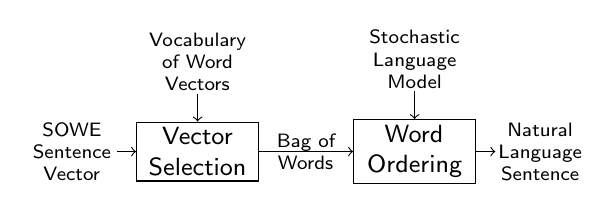
\begin{tikzpicture}[
	every node/.style={ text width=4em,
    					align=center,
                        font=\scriptsize\sffamily,
                        inner sep=1pt
                        },
	proc/.style= {draw,
    			  font=\small\sffamily,
                  inner sep = 2pt
    }
]
	\node (input) [inner sep=-4pt] {SOWE Sentence Vector};
    \node (selection) [proc, right = 0.7em of input]{Vector\\ Selection};
    \node (ordering) [proc, right = 3.4em of selection]{Word\\ Ordering};
	\node (vocab) [above = 1em of selection]{Vocabulary of Word Vectors};
    \node (lm) [above = 1em of ordering] {Stochastic Language Model};
    \node (output) [inner sep=-4pt, right=0.7em of ordering] {Natural Language Sentence};
    \draw[->] (input) -- (selection);
    \draw[->] (vocab) -- (selection);
    \draw[->] (selection) -- (ordering) node[midway] {Bag of Words};
    \draw[->] (lm) -- (ordering);
    \draw[->] (ordering) -- (output);
\end{tikzpicture}

\end{document}
	\caption{The \twosteptitle{} process for the regenerating sentences from SOWE-type sentence vectors.}
	\label{block_diagram}
\end{figure}

The rest of the paper is organized into the following sections. \Cref{relwork} discusses the prior work on sentence  generation. \Cref{framework} explains the problem in detail and how our method is used to solve it. \Cref{evalsettings} describes the settings used for evaluation. \Cref{resultsSS} presents the results of this evaluation. The paper concludes with \Cref{conclusionSS} and a discussion of future work on this problem.


\section{Related Works}\label{relwork}


To the best of our knowledge only three prior works exist in the area of sentence generation from embeddings. The first two (\textcite{Dinu2014CompositionalGeneration}, \textcite{iyyer2014generating}) are based on the recursive structures in language, while \textcite{Bowman2015SmoothGeneration}, uses the sequential structure.


\renewcommand{\u}{\tilde{u}}

%\subsubsection{Compositional Sentence Generation}
\textcite{Dinu2014CompositionalGeneration}  extends the models described by \textcite{zanzotto2010estimating} and \textcite{Guevara2010} for generation. The composition is described as a linear transformation of the input word embeddings to get an output vector, and another linear transformation to reverse the composition reconstructing the input. The linear transformation matrices are solved using least squares regression. This method of composing, can be applied recursively from words to phrases to clauses and so forth.
It theoretically generalises to whole sentences, by recursively applying the composition or decomposition functions. However, Dinu and Baroni's work is quantitatively assessed only on direct reconstruction for decomposing Preposition-Noun and Adjective-Noun word phrases. In these cases where the decomposition function was trained directly on vectors generated using the dual composition function they were able to get perfect reconstruction on the word embedding based inputs.
% -- though as they note, this is not extremely difficult as it is fitting linear transformation to invert a linear transformation.


\textcite{iyyer2014generating} extends the work of \textcite{SocherEtAl2011:PoolRAE} defining an unfolding recursive dependency-tree recursive autoencoder (DT-RAE). Recursive neural networks are jointly trained for both composing the sentence's words into a vector, and for decomposing that vector into words. This composition and decomposition is done by reusing a composition neural network at each vertex of the  dependency tree structure, with different weight matrices for each dependency relation. The total network is trained based on the accuracy of reproducing its input word embeddings. It can be used to generate sentences, if a dependency tree structure for the output is provided. This method was demonstrated quantitatively on five examples; the generated sentences were shown to be loosely semantically similar to the originals.


\textcite{Bowman2015SmoothGeneration} uses a a modification of the variational autoencoder (VAE) \parencite{2014VAE} with natural language inputs and outputs, to learn the sentence representations. These input and output stages are performed using long short-term memory recurrent neural networks \parencite{hochreiter1997long}. They demonstrate a number of uses of this technique, one of which is sentence generation, in the sense of this paper.
While Bowman et al. do define a generative model, they do not seek to recreate a sentence purely from its vector input, but rather to produce a series of probability distributions on the words in the sentence. These distributions can be evaluated greedily, which the authors used to give three short examples of resynthesis. They found the sentence embeddings created captured largely syntactic and loose topical information. 

We note that none of the aforementioned works present any quantitative evaluations on a corpus of full sentences. We suggest that that is due to difficulties in evaluation. As noted in \textcite{iyyer2014generating} and \textcite{Bowman2015SmoothGeneration}, they tend to output lose paraphrases, or roughly similar sentences. This itself is a separately useful achievement to pure exact sentence generation; but it is not one that allows ready interpretation of how much information is maintained by the embeddings. Demonstration of our method at generating the example sentences used in those work is available as supplementary material\footnote{\url{http://white.ucc.asn.au/publications/White2016SOWE2Sent/}}. As our method often can exactly recreate the original sentence from its vector representation evaluation is simpler.

Unlike current sentence generation methods, the non-compositional BOW generation method of \textcite{White2015BOWgen} generally outputs a BOW very close to the reference for that sentence -- albeit at the cost of losing all word order information. It is because of this accuracy that we base our proposed sentence generation method on it (as detailed in \Cref{selection}). The word selection step we used is directly based on their greedy BOW generation method. We improve it for sentence generation by composing with a word ordering step to create the sentence generation process.



\section{General Framework}\label{framework}
As discussed in \Cref{intro}, and shown in \Cref{block_diagram}, the approach taken to generate the sentences from the vectors comes in two steps. First selecting the words used -- this is done deterministically, based on a search of the embedding space. Second is to order them, which we solve by finding the most likely sequence according to a stochastic language model. Unlike the existing methods, this is a deterministic approach, rather than a machine learn method. The two subproblems which result from this split resemble more classical NP-Hard computer science problems; thus variations on known techniques can be used to solve them.

\subsection{Word Selection} \label{selection}
\renewcommand{\c}{\tilde{c}}
\newcommand{\s}{\tilde{s}}
\newcommand{\x}{\tilde{x}}
\renewcommand{\t}{\tilde{t}}
\newcommand{\N}{\mathbb{N}}
\newcommand{\R}{\mathbb{R}}
\newcommand{\V}{\mathcal{V}}
\def\B{\mathcal{B}}




\textcite{White2015BOWgen} approaches the BOW generation problem, as task of selecting the vectors that sum to be closest to a given vector. This is related to the knapsack and subset sum problems. They formally define the vector selection problem as:
\[
(\s,\V,\,d) \mapsto \argmin_{\left\{ \forall\c\in\N_{0}^{|\V|}\right\} }\:d( \s,\,\sum_{\x_j\in\V}\:\x_{j}c_{j})
\]
to find the bag of vectors selected from the vocabulary set $\V$ which when summed is closest to the target vector $\s$. Closeness is assessed with distance metric $d$. $\c$ is the indicator function for that multi-set of vectors. As there is a one to one correspondence between word embeddings and their words, finding the vectors results in finding the words. \textcite{White2015BOWgen} propose a greedy solution to the problem\footnote{We also investigated beam search as a possible improvement over the  greedy addition and $n$-substitution  used by \textcite{White2015BOWgen}, but did not find significant improvement. The additional points considered by the beam tended to be words that would be chosen by the greedy addition in the later steps -- thus few alternatives where found.}.

The key algorithm  proposed by \textcite{White2015BOWgen} is greedy addition. The idea is to greedily add vectors to a partial solution building towards a complete bag. This starts with an empty bag of word embeddings, and at each step the embedding space is searched for the vector which when added to the current partial solution results in the minimal distance to the target -- when compared to other vectors from the vocabulary. This step is repeated until there are no vectors in the vocabulary that can be added without moving away from the solution. Then a fine-tuning step, $n$-substitution, is used to remove some simpler greedy mistakes.

The $n$-substitution step examines partial solutions (bags of vectors) and evaluates if it is possible to find a better solution by removing $n$ elements and replacing them with up-to $n$ different elements. The replacement search is exhaustive over the $n$-ary Cartesian product of the vocabulary. Only for $n=1$ is it currently feasible for practical implementation outside of highly restricted vocabularies. Never-the-less even $1$-substitution can be seen as lessening the greed of the algorithm, through allowing early decisions to be reconsidered in the full context of the partial solution. The algorithm does remain greedy, but many simple mistakes are avoided by $n$-substitution. The greedy addition and $n$-substitution processes are repeated until the solution converges.



\subsection{The Ordering Problem} \label{ordering}
\begin{figure*}
	\resizebox{\textwidth}{!}{\documentclass{standalone}
\usepackage{arrayjobx}
\usepackage{xifthen}
\usepackage{tikz,textcomp}
\usepackage{ amssymb }

\begin{document}
	
\tikzset{ shorten <>/.style={ shorten >=0.2cm, shorten <=0.2cm } }

\begin{tikzpicture}
\newarray\Words
\readarray{Words}{$w_\triangleright$&$w_1$&$w_2$&$w_3$&$w_4$&$w_\triangleleft$}
\dataheight=5

\newcommand{\ystep}{0.5}

\newcommand{\gx}{}
\newcommand{\gy}{}


\newcommand{\drawgroupinner}{
	\foreach \j in {1,...,6}
	{
		\colorlet{MyColor}{black}%
		\ifthenelse{\i=\j}{\colorlet{MyColor}{gray}}{}
		\ifthenelse{\j=1}{\colorlet{MyColor}{gray}}{}
		
		\node[MyColor] (w_\i\j) at (\gx,\gy-\ystep*\j cm) {\Words(\i)\Words(\j)};
	}
	\draw (\gx,\gy-3.5*\ystep cm) ellipse (0.7cm and \ystep*4 cm);
}

\newcommand{\drawgrouptop}[3]{%
	\renewcommand{\i}{#1}
	\renewcommand{\gx}{#2 cm}
	\renewcommand{\gy}{#3 cm}
	\drawgroupinner{}	
	\node at (\gx,\gy+1*\ystep cm) {$S($\Words(\i)$)$};

}
\newcommand{\drawgroupbottom}[3]{%
	\renewcommand{\i}{#1}
	\renewcommand{\gx}{#2 cm}
	\renewcommand{\gy}{#3 cm}
	\drawgroupinner{}	
	\node at (\gx,\gy-8*\ystep cm) {$S($\Words(\i)$)$};	
}



\drawgrouptop{1}{0}{0}
\drawgrouptop{2}{2.5}{2.5}
\drawgroupbottom{3}{5}{-1.5}
\drawgrouptop{4}{7.5}{2.5}
\drawgrouptop{5}{10}{0}



\foreach \i in {1,...,5}
{	
	\foreach \j in {2,...,5}
	{
		\colorlet{MyColor}{black}%
		\ifthenelse{\j=2}{\colorlet{MyColor}{cyan!50!black}}
		{\ifthenelse{\j=3}{\colorlet{MyColor}{blue!50!black}}%
%		{\ifthenelse{\j=3}{\colorlet{MyColor}{red!50!black}}%
		{\ifthenelse{\j=4}{\colorlet{MyColor}{yellow!50!black}}%
		{\ifthenelse{\j=5}{\colorlet{MyColor}{green!50!black}}%
		{}}}}%}


		\ifthenelse{ \NOT \i=\j}{
			\foreach \k in {2,...,6}
			{
				\ifthenelse{\NOT \k=\i \AND \NOT \k=\j}
				{
					\draw[->,MyColor] (w_\i\j) -- (w_\j\k);
				}{}
			}
		}{}
	}
}

\node (w_S) at (-2cm,-1.5) {$w_\blacktriangleright$\Words(1)};
\draw (-2cm,-1.5) ellipse (0.7cm and 1 cm);
\node at (-2cm,-1.5cm +1.3 cm) {$S(w_\blacktriangleright)$};


\foreach \j in {2,...,5}
{
	\draw[->, red!70!black] (w_S)  --  (w_1\j);
}


\node (w_E) at (12cm,-1.5) {\Words(6)$w_\blacktriangleleft$};
\draw (12cm,-1.5) ellipse (0.7cm and 1 cm);
\node at (12cm,-1.5cm +1.3 cm) {$S($\Words(6)$)$};
\foreach \j in {1,...,5}
{
	\draw[->, red!70!black] (w_\j6) -- (w_E);
}

%\draw[->,line width=1mm,brown] (w_S) -- (w_12) -- (w_23)--(w_34)--(w_45)--(w_56)--(w_E);

\end{tikzpicture}

\end{document}}
	\caption{\label{fig:ordergraph} A graph showing the legal transitions between states, when the word-ordering problem is expressed similar to a GA-TSP. Each edge $\langle w_{a},w_{b}\rangle \to \langle w_{c},w_{d}\rangle$  has cost $-\log(P(w_c\:|\:w_aw_b)$. The nodes are grouped into districts (words). Nodes for invalid states are greyed out.} 
\end{figure*}

After the bag of words has been generated by the previous step, it must be ordered (sometimes called linearized). For example ``are how , today hello ? you'', is to be ordered into the sentence: ``hello , how are you today ?''. This problem cannot always be solved to a single correct solution. \textcite{Mitchell2008}  gives the example of ``It was not the sales manager who hit the bottle that day, but the office worker with the serious drinking problem.'' which has the same word content (though not punctuation) as ``That day the office manager, who was drinking, hit the problem sales worker with a bottle, but it was not serious.''. However, while a unique ordering cannot be guaranteed, finding the most likely word ordering is possible. There are several current methods for word ordering

To order the words we use a method based on the work of \textcite{Horvat2014}, which uses simple trigrams. More recent works, such as beam-search and LSTM language model and proposed by \textcite{2016arXiv160408633S}; or a syntactic rules based method such as presented in \textcite{ZhangWordOrderSyntax}, could be used. These more powerful ordering methods internalise significant information about the language. The classical trigram language model we present is a clearer baseline for the capacity to regenerate the sentences; which then be improved by using such systems.

\textcite{Horvat2014} formulated the word ordering problem as a generalised asymmetrical travelling salesman problem (GA-TSP). \Cref{fig:ordergraph} shows an example of the connected graph for ordering five words. We extend beyond the approach of \textcite{Horvat2014} by reformulating the problem as a linear mixed integer programming problem (MIP). This allows us to take advantage of existing efficient solvers for this problem. 
Beyond the GA-TSP approach, a direct MIP formulation allows for increased descriptive flexibility and opens the way for further enhancement. Some of the constraints of a GA-TSP can be removed, or simplified in the direct MIP formulation for word ordering.  For example, word ordering does have distinct and known start and end nodes (as shall be detailed in the next section). To formulate it as a GA-TSP it must be a tour without beginning or end. \textcite{Horvat2014} solve this by simply connecting the start to the end with a zero cost link. This is not needed if formulating this as a MIP problem, the start and end nodes can be treated as special cases. Being able to special case them as nodes known always to occur allows some simplification in the subtour elimination step. The formulation to mixed integer programming is otherwise reasonably standard.

\input{pubSOWE2sent-word_ordering.tex}


\section{Experimental Setup and Evaluations} \label{evalsettings}
This experimental data used in this evaluation was
obtained from the data released with \textcite{White2015BOWgen}.\footnote{Available online at \url{http://white.ucc.asn.au/publications/White2016BOWgen/}}
\subsection{Word Embeddings}
GloVe representations of words are used in our evaluations \parencite{pennington2014glove}. GloVe was chosen because of the availability of a large pre-trained vocabulary of vectors.\footnote{Available online at \url{http://nlp.stanford.edu/projects/glove/}} The representations used for evaluation were pretrained on the 2014 Wikipedia and Gigaword 5.  Other vector representations are presumed to function similarly.
\textcite{White2015BOWgen} showed that their word selection method significantly improves with higher dimensional embeddings. Due to their findings, we only evaluated 300 dimensional embeddings.

\subsection{Corpus and Language Modelling}
\begin{figure}
	\begin{tikzpicture}
	\begin{axis}[resplot,height=0.55\columnwidth,
	ybar, ymin=0, ytick={0,1000,2000, 3000,4000,5000},
	bar width=1,
	ylabel=Number of Sentences,
	]
	\addplot table [y=Instances,x=ground_length]{\ordlenscores};
	
	\end{axis}
	\end{tikzpicture}
	\caption{\label{fig:corpus} The distribution of the evaluation corpus after preprocessing.}
\end{figure}

The evaluation was performed on a subset of the Books Corpus \parencite{moviebook}. The corpus was preprocessed as in the work of \textcite{White2015BOWgen}. This meant removing any sentences which used words not found in the embedding vocabulary.

After preprocessing, the base corpus, was split 90:10. 90\% (59,694,016 sentences) of the corpus was used to fit a trigram model. This trigram language model was smoothed using the Knesler-Ney back-off method \parencite{kneser1995improved}. The remaining 10\% of the corpus was kept in reserve. From the 10\%, 1\% (66,464 sentences) were taken for testing. From this any sentences with length over 18 words were discarded -- the time taken to evaluate longer sentences increases exponentially and becomes infeasible. This left a final test set of 53,055 sentences. \Cref{fig:corpus} shows the distribution of the evaluation corpus in terms of sentence length.
 
Note that the Books corpus contains many duplicate common sentences, as well as many duplicate books: according to the distribution site\footnote{\url{http://www.cs.toronto.edu/~mbweb/}} only 7,087 out of 11,038 original books in the corpus are unique. We did not remove any further duplicates, which means there is a strong chance of a small overlap between the test set, and the set used to fit the trigrams.
 

\subsection{Mixed Integer Programming}
Gurobi version 6.5.0 was used to solve the MIP problems, invoked though the JuMP library \parencite{jump}. During preliminary testing we found Gurobi to be significantly faster than the open source GLTK. Particularly for longer sentences, we found two orders of magnitude difference in speed for sentences of length 18. This is inline with the more extensive evaluations of \textcite{meindl2012analysis}. Gurobi was run under default settings, other than being restricted to a single thread. Restricting the solver to a single thread allowed for parallel processing.

%Processing was carried out on an AMD Opteron 6300 virtual machine with 45GB of RAM. 
Implementation was in the Julia programming language \parencite{Julia}. The implementation, and non-summarised results are available for download.\footnote{\url{http://white.ucc.asn.au/publications/White2016SOWE2Sent/}}



\section{Results and Discussion} \label{resultsSS}

\begin{table}[t]
	\centering
%	\resizebox{\linewidth}{!}{
		\setlength{\tabcolsep}{3pt}
		\pgfplotstabletypeset[col sep=comma, ignore chars={"}, fixed zerofill, precision=3,column type=C{4.5em},
		columns/Perfect Sentences/.style={percent style, precision=1},
		columns/Portion Feasible/.style={percent style, precision=1},
		every head row/.style={
			after row=\midrule
		},
		columns={Process, Perfect Sentences, BLEU Score, Portion Feasible}
		]{data/ordering_scores.csv}
	%}
	\caption{The overall performance of the \twosteptitle{} sentence generation process when evaluated on the Books corpus. }
	\label{table:overallSS}
\end{table}
\begin{table}	
	\centering
%	\resizebox{\linewidth}{!}{
		\setlength{\tabcolsep}{3pt}
		\pgfplotstabletypeset[skip rows between index={0}{4},
		col sep=comma,fixed zerofill, precision=3,column type=C{4.5em},
		columns/Perfect BOWs/.style={percent style, precision=1},
		every head row/.style={after row=\midrule},
		create on use/Process/.style={create col/set list={0,0,0,0,Word Selection}},
		columns={Process, Perfect BOWs, Mean Precision,Mean Jaccard Index}
		]{data/sowe2sent_selection_overall_len_scores.csv}
%	}
	\caption{ The performance of the word selection step, on the Books corpus. This table shows a subset of the results reported by \textcite{White2015BOWgen}.}
	\label{table:wordselection}
\end{table}


\begin{figure}
	\centering
	\pgfplotstablecreatecol[copy column from table={\sellenscores}{books_0_01_glove300_perfect_mean}] {select error} {\ordlenscoresoracle}
	\begin{tikzpicture}
	\begin{axis}[resplot,
	legend style={at={(0.02,0.02)},anchor=south west},
	xmin=0,xmax=20, xtick={0,2,4,6,8,10,12,14,16,18},
	ylabel=Portion Perfect,
	cycle list name=exotic]
	\addplot table [y=Perfect Sentences,x=ground_length]{\ordlenscores};
	\addplot table [y=Perfect Sentences,x=ground_length]{\ordlenscoresoracle};
	\addplot[mark=triangle*] table [y=books_0_01_glove300_perfect_mean ,x=ground_len,
					skip coords between index={18}{1000}, 		
	]{\sellenscores};
	
	\legend{\twosteptitle{}, \oracletitle{}, \selectiontitle{}}
	\end{axis}
	\end{tikzpicture}
	\caption{The portion of sentences reconstructed perfectly by the \twosteptitle{} process. Shown also is the results on ordering only (\oracletitle{}), which orders the reference BOWS; and the portion of BOWs perfect from the word selection step only (\selectiontitle{}) i.e. the input to the ordering step.}
	\label{figure:exactlenscoreSS}
\end{figure}


The overall results for our method (\twosteptitle{}) sentence generation are shown in \Cref{table:overallSS}. Also shown are the results for just the ordering step, when the reference bag of words provided as the input (\oracletitle{}). The Perfect Sentences column shows the portion of the output sentences which exactly reproduce the input. The more forgiving BLEU Score \cite{Papineni2002} is shown to measure how close the generated sentence is to the original. The portion of cases for which there does exist a solution within the constraints of the MIP ordering problem is showin in Portion Feasible. In the other cases, where the MIP problem is unsolvable, for calculating the BLEU score, we order the BOW based on the order resulting from the word selection step, or in the reference case randomly.

\Cref{table:wordselection} shows the results reported by \cite{White2015BOWgen} for the Word Selection step only (\selectiontitle{}). The Perfect BOWs column reports the portion of the generated BOWs which perfectly match the reference BOWs. We also show the Mean Precision, averaged across all cases, this being the number of correct words generated, out of the total number of words generated. Similarly, the Mean Jaccard Index is shown, which is a measure of the similarities of the BOWs, being the size of the intersection of the generated BOW with the reference BOW, divided by the size of their union. We present these results to show how each step's performance impacts the overall system.


Both the \oracletitle{} and \selectiontitle{} results place an upper bound on the performance of the overall approach (\twosteptitle{}). The ordering only results (\oracletitle{}) show the best performance that can be obtained in ordering with this language model, when no mistakes are made in selection. Similarly, the selection only results (\selectiontitle{}) are bounding as no matter how good the word ordering method is, it cannot recreate perfectly accurate sentences using incorrect words.


It can be noted that \oracletitle{} and \twosteptitle{} were significantly more accurate than the best results reported by \textcite{Horvat2014}. We attribute this to Horvat and Byrne preprocessing the evaluation corpora to remove the easier sentences with 4 or less words. We did not remove short sentences from the corpus. The performance on these sentences was particularly high, thus improving the overall results on ordering.



The overall resynthesis (\twosteptitle{}) degrades as the sentence length increases as shown in \Cref{figure:exactlenscoreSS}. It can be seen from the figure that sentence length is a critical factor in the performance. The performance drop is largely from the complexity in the ordering step when faced with long sentences. This is evident in \Cref{figure:exactlenscore}, as performance degrades at almost the same rate even when using the perfect BOW (compare \oracletitle{} vs \twosteptitle{}); rather than being degraded by the failures in the word selection step (\selectiontitle{}). We can conclude that sentences with word selection failures (\selectiontitle{}) are also generally sentences which would have word ordering failures even with perfect BOW (\oracletitle{}). Thus improving word selection, without also improving ordering, would not have improved the overall results significantly.

From observing examples of the output of method we note that normally mistakes made in the word selection step result in an unorderable sentence. Failures in selection are likely to result in a BOW that cannot be grammatically combined e.g. missing conjunctions. This results in no feasible solutions to the word ordering problem.


Our method considers the word selection and word ordering as separate steps. This means that unorderable words can be selected if there is an error in the first step. This is not a problem for the existing methods of \textcite{iyyer2014generating} and of \textcite{Bowman2015SmoothGeneration}. \textcite{iyyer2014generating} guarantees grammatical correctness, as the syntax tree must be provided as an input for resynthesis -- thus key ordering information is indirectly provided and it is generated into. \textcite{Bowman2015SmoothGeneration} on the other hand integrates the language model with the sentence embedding so that every point in the vector space includes information about word order. In general, it seems clear that incorporating knowledge about order, or at least co-occurrence probabilities, should be certain to improve the selection step. Even so the current simple approach has a strong capacity to get back the input, without such enhancement.


\section{Conclusion} \label{conclusionSS}
A method was presented for regenerating sentences, from the sum of a sentence's word embeddings. It uses sums of existing word embeddings, which are machine learnt to represent the sentences, and then generates natural language output, using only the embeddings and a simple trigram language model. Unlike existing methods, the generation method itself is deterministic rather than being based on machine-learnt encoder/decoder models. The method involved two steps, word selection and word ordering.

The first part is  the word selection problem, of going from the sum of embeddings to a bag of words. To solve this we utilised the method presented in \textcite{White2015BOWgen}. Their greedy algorithm was found to perform well at regenerating a BOW. The second part was word ordering. This was done through a MIP bases reformulation of the work of the graph-based work of \textcite{Horvat2014}. It was demonstrated that a probabilistic language model can be used to order the bag of words output to regenerate the original sentences. While it is certainly impossible to do this perfectly in every case, for many sentences the most likely ordering is correct.

From a theoretical basis the resolvability of the selection problem, presented by \textcite{White2015BOWgen}, shows that adding up the word embeddings does preserve the information on which words were used; particularly for higher dimensional embeddings. This shows clearly that collisions do not occur (at least with frequency) such that two unrelated sentences do not end up with the same SOWE representation. 
This work extends that by considering if the order can be recovered based on simple corpus statistics. Its recoverability is dependent, in part, on how frequent sentences with the same words in different order are in the corpus language -- if they were very frequent then non-order preserving, non-compositional representations like SOWE would be poor at capturing meaning, and the ordering task would generally fail. As the method we presented generally does succeed, we can conclude that word order ambiguity is not a dominating problem. This supports the use of simple approaches like SOWE as a meaning representation for sentences -- at least for sufficiently short sentences.

The technique was only evaluated on sentences with up to 18 words (inclusive), due to computational time limitations. Both accuracy and running time worsens exponentially as sentence length increases. With that said, short sentences are sufficient for many practical uses. For longer sentences, it is questionable as to the extent the information used is preserved by the SOWE representation -- given they tend to have large substructures (like this one) compositional models are expected to be more useful. In evaluating such future representations, the method we present here is a useful baseline.

\subsection{Acknowledgements}
This research is supported by the Australian Postgraduate
Award, and partially funded by Australian Research Council grants
DP150102405 and LP110100050. Computational resources were provided by the National eResearch Collaboration Tools and Resources project (Nectar).

%\bibliography{master}

\section{Supplementary Materials to Modelling Sentence Generation from Sum of Word Embedding Vectors as a Mixed Integer Programming Problem}
\newcommand{\cmark}{\ding{51}}%
\newcommand{\xmark}{\ding{55}}%\\
\newcommand{\namark}{\ding{54}}
\newcommand{\passmark}{--}

These supplementary materials show additional examples of the performance of our method against the works of \textcite{iyyer2014generating, Bowman2015SmoothGeneration}, as of our well as on sentences with ambiguous order. Bare in mind, exact reproduction is not the goal of either prior work; nor truly is it a goal of out work. Our goal being the regeneration of sentences while preserving meaning -- exact reproduction does of course meet that goal. The examples that follow should highlight the differences in the performance of the methods.





\Cref{egiyyer,egbowman,egordered} show quantitative examples; including comparison to the existing works. In these tables \xmark{} and \cmark{} are used to show correctness of the output in the selection (Sel.) and in the ordering (Ord.) steps.

The sentences shown in \Cref{egiyyer}, are difficult. The table features long complex sentences containing many proper nouns. These examples are sourced from \textcite{iyyer2014generating}. The output from their DT-RAE method is also shown for contrast. Only 3C is completed perfectly by our method. Of the remainder the MIP word ordering problem has no solutions, except in 3D, where it is wrong, but does produce an ordered sentence. In the others the language model constraints does not return any feasible ($P(\tau)>0$) ordering solutions. This failure may be attributed in a large part to the proper nouns.  Proper nouns are very sparse in any training corpus for language modelling. The Kneser-Ney smoothed trigrams back-off only down to bigrams, so if the words of the bigrams from the training corpus never appear adjacently in the training corpus, ordering fails. This is largely the case for very rare words. The other significant factor is the sentence length.

The sentences in \Cref{egbowman}, are short and use common words -- they are easy to resynthesis. These examples come from \textcite{Bowman2015SmoothGeneration}. The output of their VAE based approach can be compared to that from our approach. Of the three there were two exact match's, and one failure.

Normally mistakes made in the word selection step result in an unorderable sentence. Failures in selection are likely to result in a BOW that cannot be grammatically combined e.g. missing conjunctions. This results in no feasible solutions to the word ordering problem.

The examples shown in \Cref{egordered} highlight sentences where the order is ambiguous -- where there are multiple reasonable solutions to the word ordering problem. In both cases the word selection performs perfectly, but the ordering is varied. In 5A, the \oracletitle{} sentence and the overall \twosteptitle{} sentence  in word order but not in word content. This is because under the trigram language model both sentences have exactly identical probabilities, so it comes to which solution is found first, which varies on the state of the MIP solver. In 5B the word order is switched -- ``from Paris to London'' vs ``to London from Paris'', which has the same meaning. But, it could also have switched the place names. In cases like this where two orderings are reasonable, the ordering method is certain to fail consistently for one of the orderings. Though it is possible to output the second (and third etc.) most probable ordering, which does ameliorate the failure somewhat. This is the key limitation which prevents this method from direct practical applications.

\newpage


	\newcommand{\collenone}{2.3cm}
	\newcommand{\collentwo}{8cm}
	\newcommand{\collenthree}{0.5cm}
	\newcommand{\reftitle}{Reference}
	\newcommand{\iref}{DT-RAE Ref.}
	\newcommand{\ip}{DT-RAE Para.}
	\newcommand{\bm}{VAE Mean}
	\newcommand{\bs}{VAE Sample}
	\begin{table*}
		\small
		\begin{tabular}{ p{\collenone} p{\collentwo} C{\collenthree} C{\collenthree} }
			
			\textbf{3A \hfill \reftitle}  & name this 1922 novel about leopold bloom written by james joyce . & \textbf{Sel.} & \textbf{Ord.} \\
			\textbf{\oracletitle}  & written by name this . novel about 1922 bloom leopold james joyce & \passmark & \namark \\
			\textbf{\twosteptitle}  & written novel by name james about leopold this bloom 1922 joyce . & \cmark & \namark \\
			\textbf{\iref}  & name this 1906 novel about gottlieb\_fecknoe inspired by james\_joyce &  &  \\
			\textbf{\ip}  & what is this william golding novel by its written writer &  &  \\
			\hline
			\textbf{3B \hfill \reftitle}  & ralph waldo emerson dismissed this poet as the jingle man and james russell lowell called him three-fifths genius and two-fifths sheer fudge . & \textbf{Sel.} & \textbf{Ord.} \\
			\textbf{\oracletitle}  & sheer this as james two-fifths emerson fudge lowell poet genius waldo called russell the and ralph and him . dismissed jingle three-fifths man & \passmark & \namark \\
			\textbf{\twosteptitle}  & him `` james great as emerson genius ralph the lowell and sheer waldo three-fifths man fudge dismissed jingle russell two-fifths and gwalchmai 2009 vice-versa \_\_\_\_\_\_\_\_\_\_\_\_\_\_\_\_\_\_\_\_\_\_\_\_\_\_\_\_\_\_\_\_\_\_\_\_\_\_\_\_\_\_\_\_ prominent called 21.25 explained & \xmark & \namark \\
			\textbf{\iref}  & henry\_david\_thoreau rejected this author like the tsar boat and imbalance created known good writing and his own death &  &  \\
			\textbf{\ip}  & henry\_david\_thoreau rejected him through their stories to go money well inspired stories to write as her writing &  &  \\
			\hline
			\textbf{3C \hfill \reftitle}  & this is the basis of a comedy of manners first performed in 1892 . & \textbf{Sel.} & \textbf{Ord.} \\
			\textbf{\oracletitle}  & this is the basis of a comedy of manners first performed in 1892 . & \passmark & \cmark \\
			\textbf{\twosteptitle}  & this is the basis of a comedy of manners first performed in 1892 . & \cmark & \cmark \\
			\textbf{\iref}  & another is the subject of this trilogy of romance most performed in 1874 &  &  \\
			\textbf{\ip}  & subject of drama from him about romance  &  &  \\
			\hline
			\textbf{3D \hfill \reftitle}  & in a third novel a sailor abandons the patna and meets marlow who in another novel meets kurtz in the congo . & \textbf{Sel.} & \textbf{Ord.} \\
			\textbf{\oracletitle}  & kurtz and another meets sailor meets the marlow who abandons a third novel in a novel in the congo in patna . & \passmark & \xmark \\
			\textbf{\twosteptitle}  & kurtz and another meets sailor meets the marlow who abandons a third novel in a novel in the congo in patna . & \cmark & \xmark \\
			\textbf{\iref}  & during the short book the lady seduces the family and meets cousin he in a novel dies sister from the mr. &  &  \\
			\textbf{\ip}  & during book of its author young lady seduces the family to marry old suicide while i marries himself in marriage &  &  \\
			\hline
			\textbf{3E \hfill \reftitle}  & thus she leaves her husband and child for aleksei vronsky but all ends sadly when she leaps in front of a train . & \textbf{Sel.} & \textbf{Ord.} \\
			\textbf{\oracletitle}  & train front of child vronsky but and for leaps thus sadly all her she she in when aleksei husband ends a . leaves & \passmark & \namark \\
			\textbf{\twosteptitle}  & she her all when child for leaves front but and train ends husband aleksei leaps of vronsky in a sadly micro-history thus , she the & \xmark & \namark \\
			\textbf{\iref}  & however she leaves her sister and daughter from former fianc\'e and she ends unfortunately when narrator drives into life of a house &  &  \\
			\textbf{\ip}  & leaves the sister of man in this novel &  &  \\
		\end{tabular}
		
		
		\caption{\label{egiyyer} A comparison our method, to the example sentences generated by the DT-RAE method of \textcite{iyyer2014generating}. \oracletitle{}  shows the word ordering step on the reference BOW. the Sel. and Ord. columns indicate if the output had the correct words selected, and ordered respectively. With \cmark{} indicating correct and \xmark{} indicating incorrect. \namark{} indicates not only that ordering was not correct, but that the MIP problem had no feasible solutions at all.
			\iref{} shows the result of the method of \textcite{iyyer2014generating}, when the dependency tree of the output is provided to the generating process, whereas in \ip{} an arbitrary dependency tree is provided to the generating process. Note that the reference used as input to \twosteptitle{} and \oracletitle{} sentence was varied slightly from that used in \textcite{iyyer2014generating} and \textcite{White2015BOWgen}, in that terminating punctuation was not removed, and nor were multiword entity references grouped into single tokens.}
	\end{table*}
	
	\renewcommand{\collenone}{2.3cm}
	\renewcommand{\collentwo}{3cm}
	\renewcommand{\collenthree}{0.5cm}
	
	\begin{table}
		\small
		
		\begin{tabular}{ p{\collenone} p{\collentwo} C{\collenthree} C{\collenthree} }
			
			\textbf{4A \hfill \reftitle}  & we looked out at the setting sun . & \textbf{Sel.} & \textbf{Ord.} \\
			\textbf{\oracletitle}  & we looked out at the setting sun . & \passmark & \cmark \\
			\textbf{\twosteptitle}  & we looked out at the setting sun . & \cmark & \cmark \\
			\textbf{\bm}  & they were laughing at the same time . &  &  \\
			\textbf{\bs 1}  & ill see you in the early morning . &  &  \\
			\textbf{\bs 2}  & i looked up at the blue sky . &  &  \\
			\textbf{\bs 3}  & it was down on the dance floor . &  &  \\
			\hline
			\textbf{4B \hfill \reftitle}  & i went to the kitchen . & \textbf{Sel.} & \textbf{Ord.} \\
			\textbf{\oracletitle}  & i went to the kitchen . & \passmark & \cmark \\
			\textbf{\twosteptitle}  & i went to the kitchen . & \cmark & \cmark \\
			\textbf{\bm}  & i went to the kitchen . &  &  \\
			\textbf{\bs 1}  & i went to my apartment .  &  &  \\
			\textbf{\bs 2}  & i looked around the room . &  &  \\
			\textbf{\bs 3}  & i turned back to the table . &  &  \\
			\hline
			\textbf{4C \hfill \reftitle}  & how are you doing ? & \textbf{Sel.} & \textbf{Ord.} \\
			\textbf{\oracletitle}  & how are you doing ? & \passmark & \cmark \\
			\textbf{\twosteptitle}  & how 're do well ? & \xmark & \xmark \\
			\textbf{\bm}  & what are you doing ? &  &  \\
			\textbf{\bs 1}  & “ are you sure ? &  &  \\
			\textbf{\bs 2}  & what are you doing, ? &  &  \\
			\textbf{\bs 3}  & what are you doing ? &  &  \\
		\end{tabular}
		
		\caption{\label{egbowman} A comparison of the output of the Two Step process proposed in this paper, to the example sentences generated by the VAE method of \textcite{Bowman2015SmoothGeneration}.}
	\end{table}
	
	
	\begin{table}
		\small
		\begin{tabular}{ p{\collenone} p{\collentwo} C{\collenthree} C{\collenthree} }
			
			\textbf{5A \hfill \reftitle}  & it was the worst of times , it was the best of times . & \textbf{Sel.} & \textbf{Ord.} \\
			\textbf{\oracletitle}  & it was the worst of times , it was the best of times . & \passmark & \cmark \\
			\textbf{\twosteptitle}  & it was the best of times , it was the worst of times . & \cmark & \xmark \\
			\hline
			\textbf{5B \hfill \reftitle}  & please give me directions from Paris to London . & \textbf{Sel.} & \textbf{Ord.} \\
			\textbf{\oracletitle}  & please give me directions to London from Paris . & \passmark & \xmark \\
			\textbf{\twosteptitle}  & please give me directions to London from Paris . & \cmark & \xmark \\
			\hline
		\end{tabular}
		\caption{    \label{egordered} A pair of example sentences, where the correct order is particularly ambiguous.}
	\end{table}
	
	
%	\section{appendix}
%	
%	\begin{frame}{Experimental Setup: we used the Brown, and the Books Corpus}
%		\footfullcite{francis1979brown}
%		\footfullcite{moviebook}
%		
%		\begin{columns}[T]
%			\begin{column}{0.5\textwidth}
%				\textbf{Brown}
%				\begin{itemize}
%					\item 40,485 unique words
%					\item 42,004 sentences
%					\item Sentence Length Q3: \\\hfill 25 words
%					\item Extracts from 500 varied works from 1961
%				\end{itemize} 
%			\end{column}
%			\begin{column}{0.5\textwidth}
%				\pause
%				\textbf{Books}
%				\begin{itemize}
%					\item 178,694 unique words
%					\item 66,464 sentences 
%					\item Sentence Length Q3: \\\hfill 17 words
%					\item 11,038 unpublished novels, we use just a small random subset
%				\end{itemize}
%			\end{column}
%		\end{columns}
%	\end{frame}


%\end{document}
}



